\section{Einleitung}

Einleitung und Fragestellung\\
\cite{houghpatent}

\subsection{Grabung Kapitol}
Grabungsverlauf bis 2014 (recherchieren)\\
Übernahme durch DAI (recherchieren)\\

\subsection{Datensatz vorstellen}
Herkunft\\
Umfang\\
Fragestellungen des Projektes\\

\subsection{Material vorstellen}

\subsubsection{Tafeln}
Die Verwendung von Tafeln zur Dokumentation von Fund- und Grabungsarealen ist in allen, im weitesten Sinne grabenden, Wissenschaften weit verbreitet. So setzt auch die Archäologie diese Methode ein. Dabei werden neben den zu dokumentierenden Gebieten verschiedenste Formen von Tafeln oder Schildern platziert, auf denen Zeit und Ort der Aufnahme sowie weitere bild- und motivbezogene Informationen festgehalten werden können. Der Vielfalt von Form und Material der Tafeln ist dabei keine Grenze gesetzt.

Bei den Tafeln, die Gegenstand dieses Projektes sind, handelt es sich um Schiefertafeln mit einem Holzrahmen, die mit Kreide beschriftet wurden (Vgl. Abb \ref{fig:einfachetafel}). Für die Detektion der Tafeln ergeben sich daraus folgende Faktoren:\\
\begin{enumerate}
\item Die Tafeln haben grundsätzlich eine rechteckige Form.
\item Durch die breite des Rahmens können bis zu zwei Rechtecke erkannt werden, ein Inneres und ein Äußeres.
\item Durch die große Differenz zwischen dem hellen Holzrahmen und der dunklen Schieferplatte sollte der innere Rand in der Regel gut detektierbar sein.
\end{enumerate}
\begin{figure}[!h]0
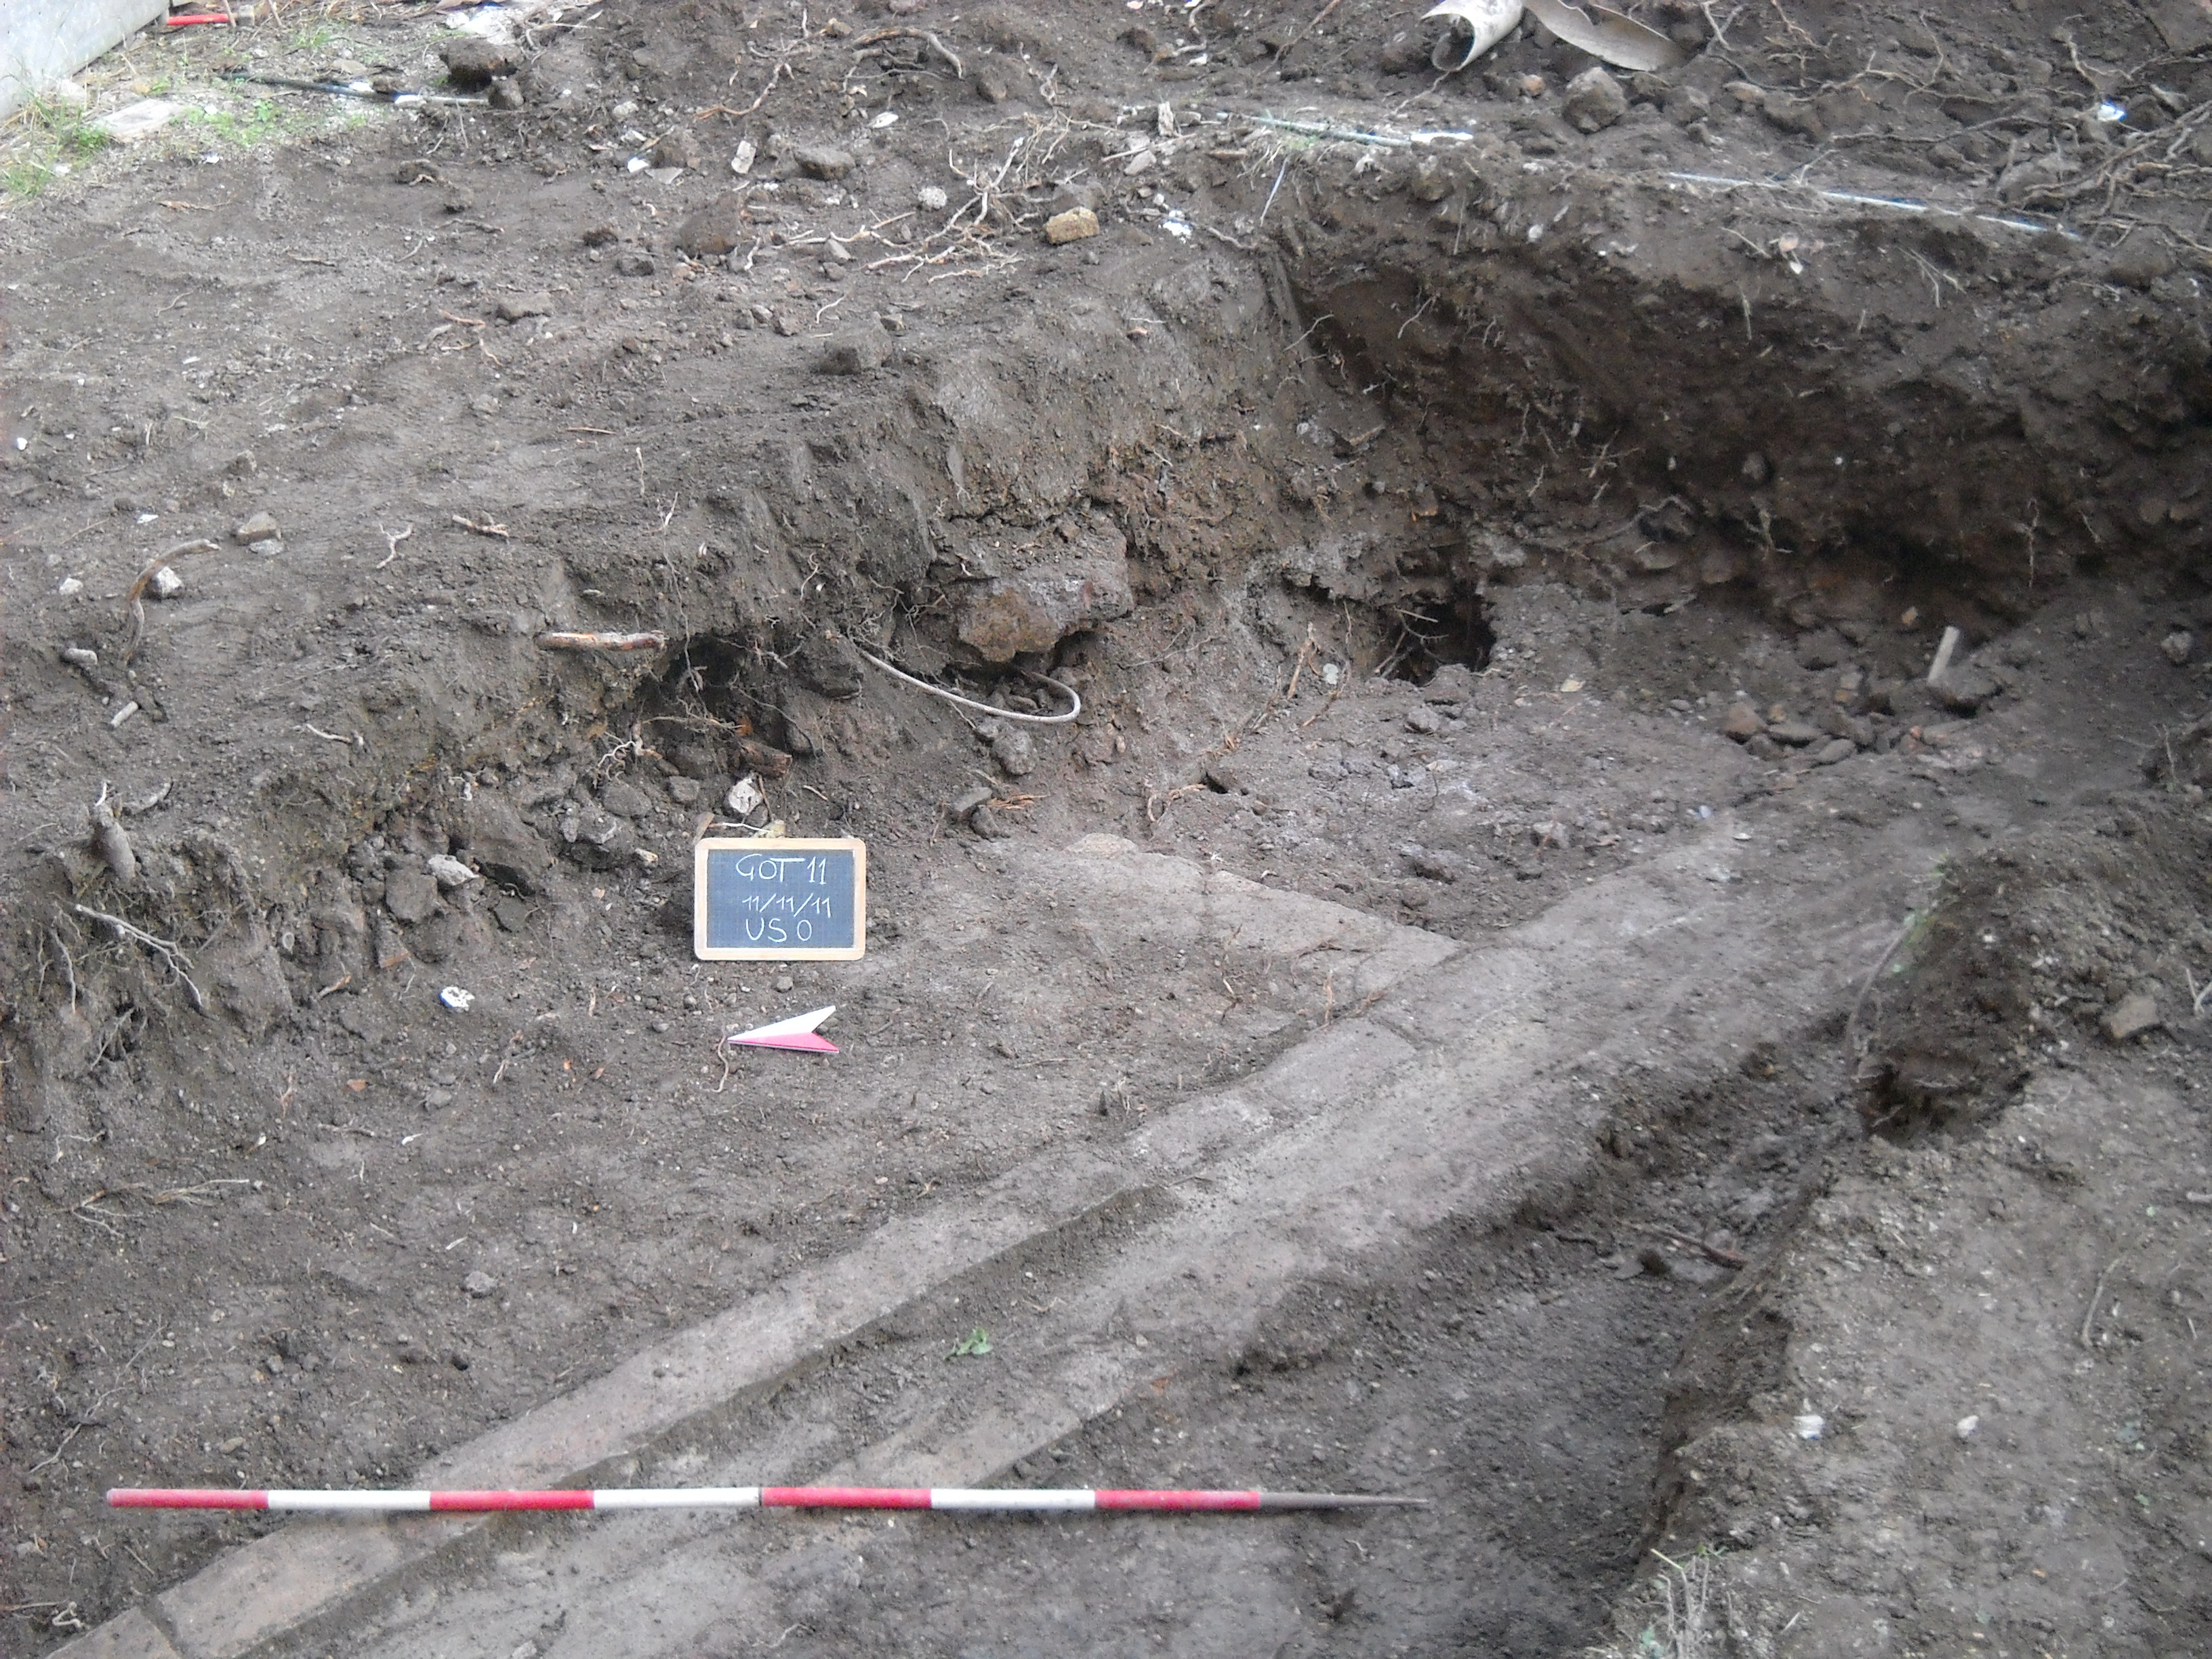
\includegraphics[width =0.5\textwidth]{catacom_1020.JPG}
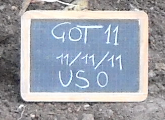
\includegraphics[width=0.5\textwidth]{catacom_1020_cutout.png}
\caption{Beispiel eines Fotos der verwendeten Tafel. GOT bezeichnet die Kampagne, darunter folgt das Datum. US ist die Abkürzung für \textit{unità stratigrafica}, die stratigrafische Einheit.}
\label{fig:einfachetafel}
\end{figure}
Die im Beispielbild gezeigte Tafel stellt  ein Idealbild dar: Die Tafel nimmt einen relativ großen Teil des Originalbildes ein. Sie ist frontal vor der Kamera positioniert. Die Beleuchtung ist gut und indirekt. Keines der weiteren Bildelemente verdeckt die Tafel.
Diese Beschreibung impliziert schon die Problemfelder, die bei der Detektion beachtet werden müssen:
\begin{enumerate}
\item Die Tafel ist unter Umständen stark rotiert (Vgl. Abb \ref{fig:schwierigetafel}).
\item Die Distanz der Tafel zur Kamera und damit ihre Größe im Bild kann stark variieren.
\item Der Rahmen der Tafel kann teilweise verdeckt oder anderweitig durch Gegenstände überlagert sein (Vgl. Abb \ref{fig:schwierigetafel}).
\item Die Farbe des Tafelrahmens kann dazu führen, dass sie sich nicht klar vom Hintergrund abhebt, was die Detektion des (äußeren) Randes erschweren kann.
\item Unregelmäßigkeiten im Rahmen, die auf grobe Verarbeitung oder Abnutzung zurückzuführen sind, können die Detektion erschweren.
\item Die Beleuchtung kann zu Problemen führen. Grundsätzlich sind alle Fotos hell und gut ausgeleuchtet, direktes Licht kann sich aber negativ auf die Kontraste auswirken.
\item Weitere Gegenstände, die den Spezifika der Tafeln entsprechen, können im Bild vorhanden sein.
\end{enumerate}
\begin{figure}[!h]
\centering
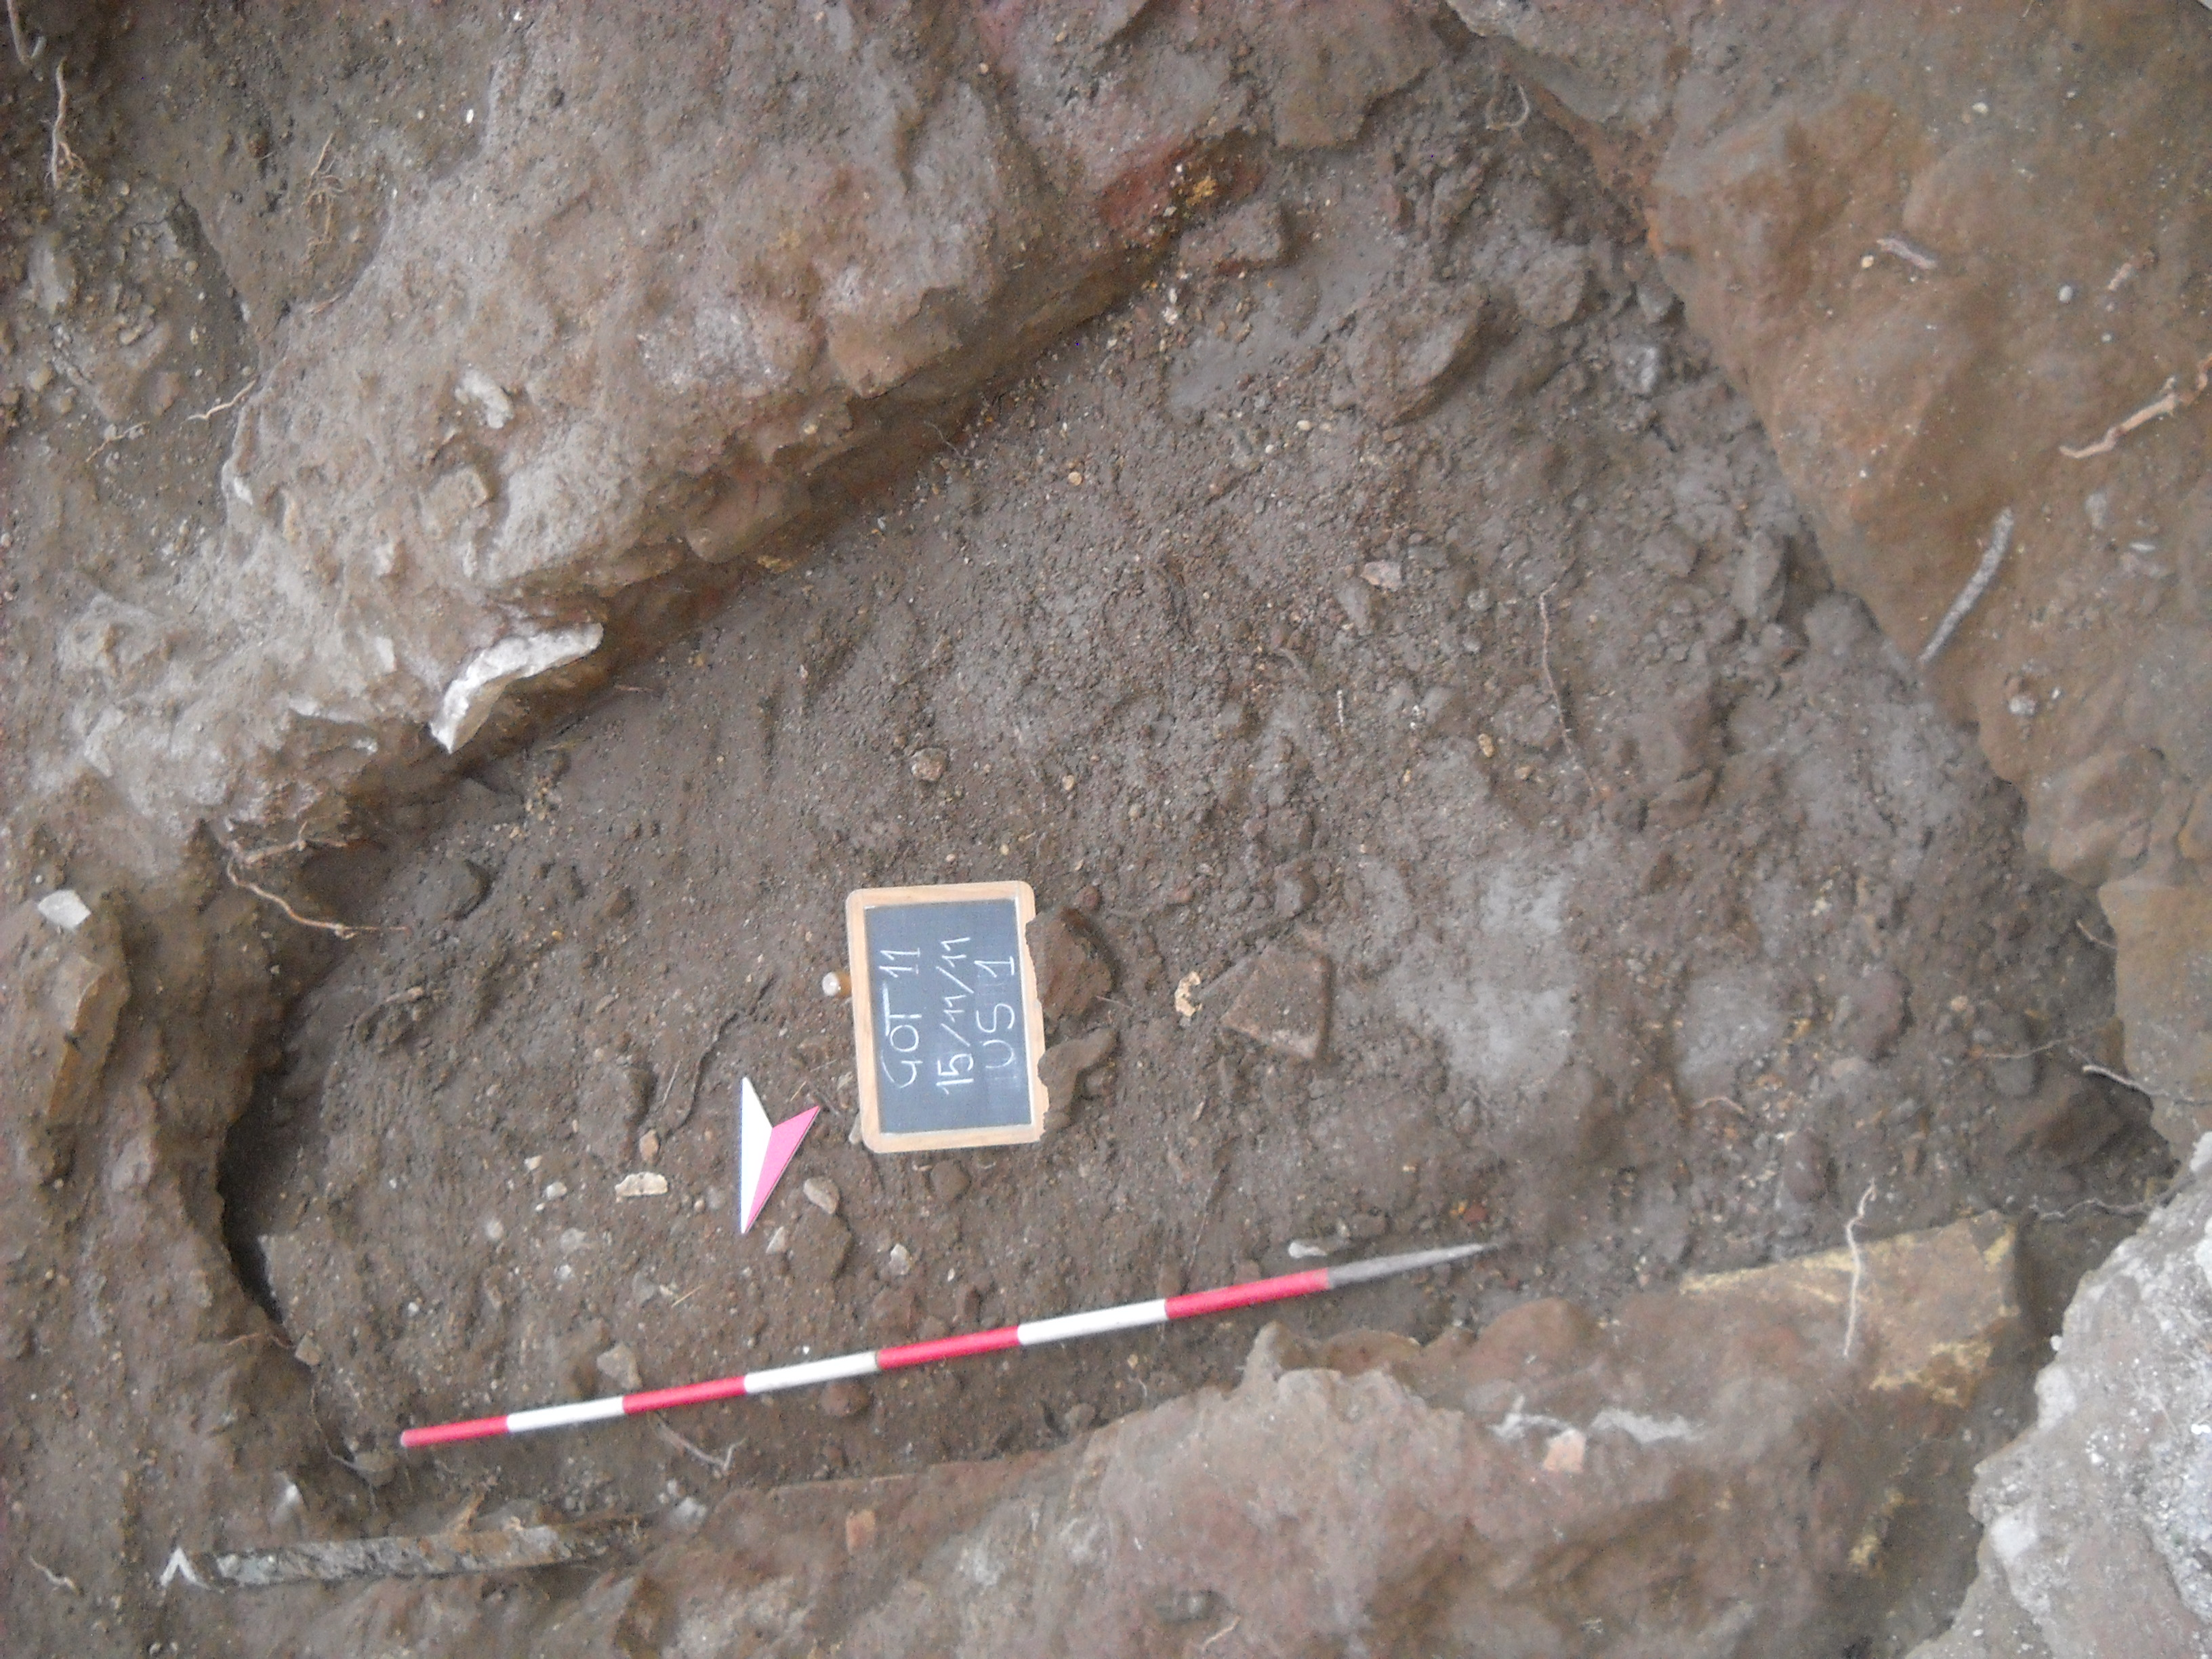
\includegraphics[width =0.5\textwidth]{catacom_1061_schwierige_tafel.JPG}
\caption{Schwierigere Detektion: Rotation und teilweise verdeckter Rahmen.}
\label{fig:schwierigetafel}
\end{figure}
Teilweise werden die hier genannten Probleme auch bei der Texterkennung wieder relevant. Auf diese und auf weitere wird an geeigneter Stelle zurückgegriffen.


\subsubsection{Tafelvergleiche}

Im Rahmen der Arbeit wurden weitere Tafeln exemplarisch dem Algorithmus unterzogen. Dabei handelte es sich um Aufnahmen der späteren Grabungen des Deutschen Archäologischen Institutes am Kapitol in Rom sowie um vergleichbare Fotos von Bodenuntersuchungen der Gruppe Terrestrische Ökohydrologie der Friedrich-Schiller-Universität Jena. Der ursprüngliche Gedanke dahinter war eine möglichst universale Detektion von Tafeln aller Art anzustreben. Die unterschiedlichen Daten konnten dabei vor allem Stärken und Schwächen der letztlich gewählten Technik aufzeigen.\\
Die Tafeln beider Projekte sollen im Folgenden kurz vorgestellt werden, um das Spektrum der Komplexität 
evtl. Vergleiche zu Tafeln aus späterer Grabung als Positivbeispiel:\\
besser gearbeitete Tafeln\\
besser lesbare Schrift\\
evtl. Vergleiche zu Tafeln der Bodenkunde als Negativbeispiel:\\
Tafel schwierig durch Form und Farbe\\
Klarsichthülle: Reflektion und Formveränderung\\
oft verdeckt\\
Bilder zur Veranschaulichung einfügen

\subsubsection{Schrift}
Kreide auf Schiefer
Probleme wie Handschrift, Verwischung, Karomuster
\subsection{Pipeline}
Struktur der Arbeit wie Pipeline:
Bildakquise
Objekterkennung
Crop-Verfahren
Pre-Processing
OCR
Evaluation
Ergebnis